\documentclass[aspectratio=35]{beamer} % Changed aspect ratio to a more vertical format

%
% Choose how your presentation looks.
%
% For more themes, color themes and font themes, see:
% http://deic.uab.es/~iblanes/beamer_gallery/index_by_theme.html
%
\mode<presentation>
{
  \usetheme{default}      % or try Darmstadt, Madrid, Warsaw, ...
  \usecolortheme{default} % or try albatross, beaver, crane, ...
  \usefonttheme{default}  % or try serif, structurebold, ...
  \setbeamertemplate{navigation symbols}{}
  \setbeamertemplate{caption}[numbered]
} 

% Set background to black and text to white
\setbeamercolor{background canvas}{bg=black}
\setbeamercolor{normal text}{fg=white}
\setbeamercolor{frametitle}{fg=white}
\setbeamercolor{title}{fg=white}

% You can continue to set other colors as needed:
\setbeamercolor{item}{fg=magenta} % Color of bullets
\setbeamercolor{subitem}{fg=yellow}
\setbeamercolor{subsubitem}{fg=cyan}
% ...
\setbeamertemplate{frametitle}[default][center]
\setbeamersize{text margin left=0.1cm, text margin right=0.1cm}
\setbeamerfont{frametitle}{size=\small}
\setbeamerfont{itemize/enumerate body}{size=\tiny}
\setbeamerfont{itemize/enumerate subbody}{size=\tiny}
\setbeamerfont{itemize/enumerate subsubbody}{size=\tiny}
\setbeamerfont{itemize/enumerate subsubsubbody}{size=\tiny}
\setlength{\leftmargini}{2.5em}  % Decrease first-level indentation
\setlength{\leftmarginii}{1em}   % Decrease second-level indentation
\setlength{\leftmarginiii}{1em} % Decrease third-level indentation

\usepackage[english]{babel}
\usepackage[utf8]{inputenc}
\usepackage[T1]{fontenc}
\usepackage{graphicx}

\usepackage{emoji}

\begin{document}

\begin{frame}
\centering
\vspace{-1in}

\includegraphics[width=0.4\textwidth]{imgs/app_icons/tiktok-icon2.png}\\
TikTok Successor Proposal \\
(Part 1 - Why)
\end{frame}

\begin{frame}{Future Videos}
\centering
\tiny
\vspace{-1.5in}
\begin{itemize}
    \item Part 1: Why replace TikTok?
    \item Part 2: Weird groupchats 
    \item Part 3: Past vertical video
    \item Part 4: Decentralization
    \item Part 5: Redesigned Algorithm
    \item Part 6: Misc / How to help
\end{itemize}
\end{frame}

\begin{frame}{Why Replace TikTok?}
\vspace{-0.4in}
\begin{itemize}
    \item Susceptible to 
    \begin{itemize}
        \item corporate greed
        \item government control 
        \begin{itemize}
            \item US Ban (bc \emoji{watermelon})
            \item China 1hr/day limit
            \item France \& Caledonia??
        \end{itemize}
    \end{itemize}
    \item Need to make nobody in charge
    \begin{itemize}
        \item Solved in Part 4
    \end{itemize}
\end{itemize}
\centering
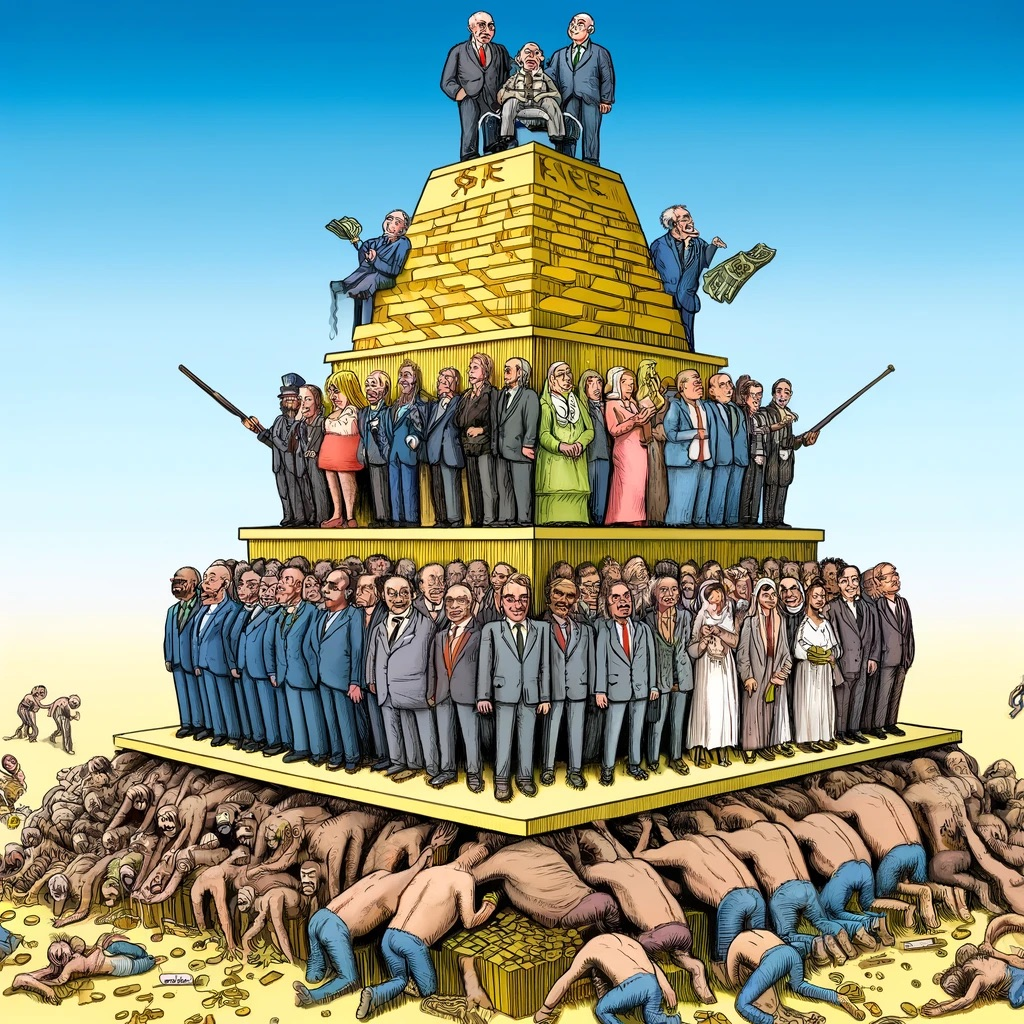
\includegraphics[width=0.8\textwidth]{imgs/why_replace/power_pyramid.jpeg}
\end{frame}

\begin{frame}{History of Communication}
\vspace{-1.1in}
\begin{enumerate}
    \item Pre-internet limited by bandwidth/access
        \begin{itemize}
            \item ex. printing press, telegram
            \item \textit{\textbf{$\uparrow$ info propagation $\rightarrow$ societal change}}
            \begin{itemize}
                \item ex. free press $\rightarrow$ India's indep
            \end{itemize}
        \end{itemize}
    \item Facebook $\rightarrow$ friends (1-to-1)
    \item YT/Insta $\rightarrow$ influencers (1-to-all \textit{for some})
    \item Reddit $\rightarrow$ interest groups (group-to-1)
    \item Tiktok $\rightarrow$ global awareness\\(all-to-1)/(1-to-all \textit{for everybody})
    \begin{itemize}\item hence \emoji{watermelon} awareness\end{itemize}
    \item We need (all-to-all), (group-to-all),\\(1-to-group), (group-to-group)
    \begin{itemize}
        \item Solved in Parts 2 \& 5
    \end{itemize}
\end{enumerate}
\end{frame}

\begin{frame}{Misinformation}
\vspace{-0.3in}
\begin{itemize}
    \item True of all social media
    \begin{itemize}
        \item Tiktok (debatably) worse
        \begin{itemize}
            \item short video $\rightarrow$ difficult to cite
            \item app difficult to navigate
        \end{itemize}
    \item AI makes this scarier
    \end{itemize}
    \item Need more media types
    \begin{itemize}
        \item Solved in Part 3
    \end{itemize}
\end{itemize}
\center

\includegraphics[width=0.8\textwidth]{imgs/why_replace/pope.png}
\end{frame}

\begin{frame}{Algorithm$\rightarrow$Echo Chamber}
\vspace{-0.6in}
\begin{itemize}
    \item True of all social media
    \begin{itemize}
        \item addiction = \$
    \end{itemize}
    \item \textit{\textbf{optionally}} expose users to diverse views
    \begin{itemize}
        \item Solved in Part 5
    \end{itemize}
\end{itemize}
\center
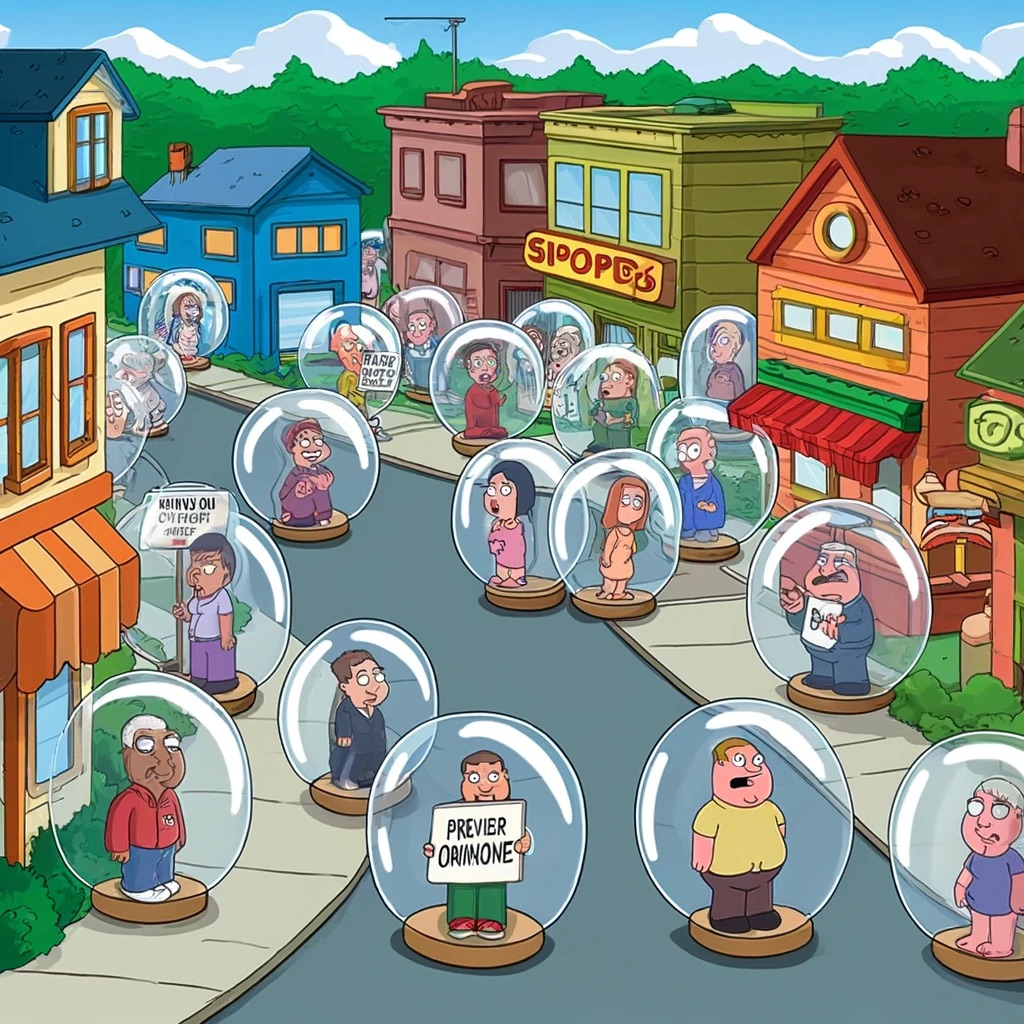
\includegraphics[width=0.8\textwidth]{imgs/why_replace/bubble_town.jpeg}
\end{frame}

\begin{frame}{Why Replace TikTok?}
\vspace{-0.7in}
\begin{itemize}
    \item Not the end of history
    \begin{itemize}
        \item Why not try to improve?
    \end{itemize}
\end{itemize}
\center
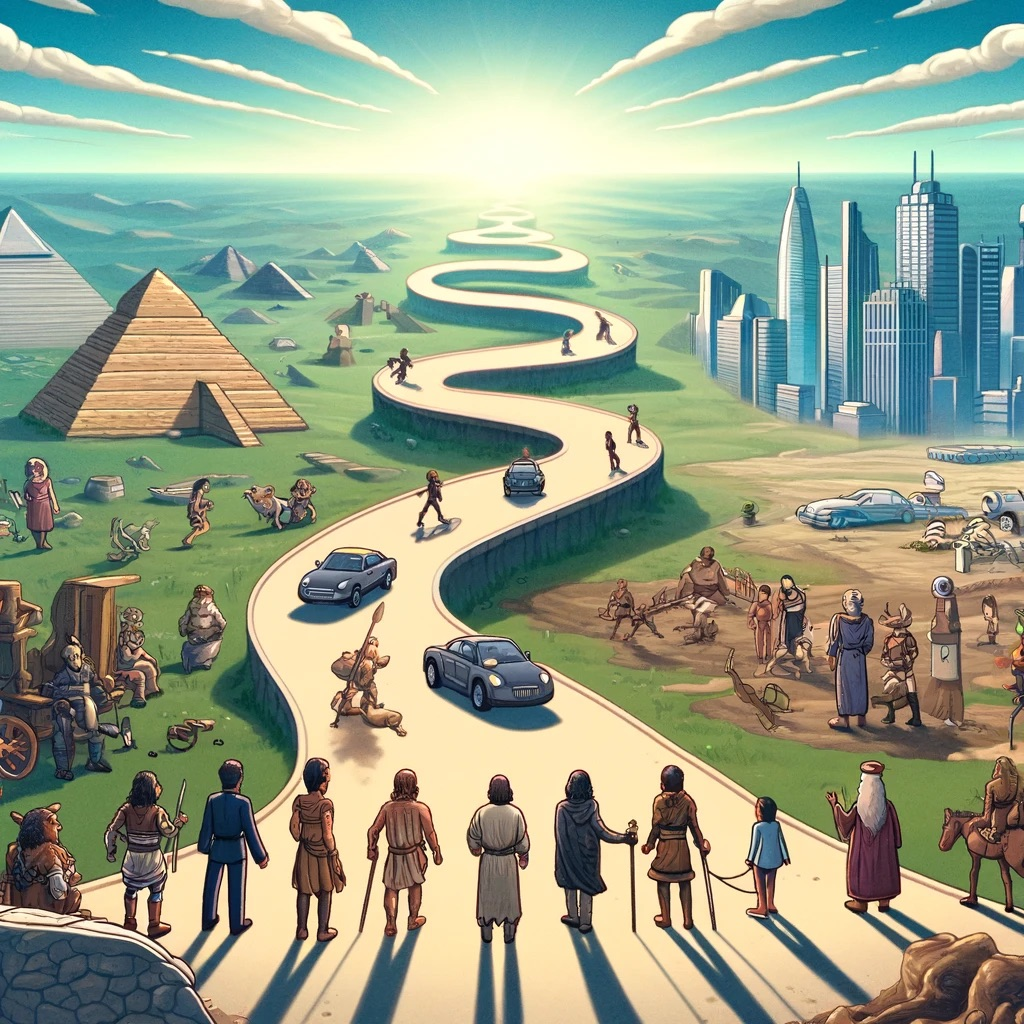
\includegraphics[width=0.8\textwidth]{imgs/why_replace/future_path.jpeg}
\end{frame}

\begin{frame}
\centering
\vspace{-1in}

\includegraphics[width=0.4\textwidth]{imgs/app_icons/tiktok-icon2.png}\\
TikTok Successor Proposal \\
(Part 2: Weird Groupchats)
\end{frame}

\begin{frame}{Human Communication\\Has A Problem}
\vspace{-0.5in}
\begin{itemize}
    \item Lots of us \& some louder than others
    \begin{itemize}
        \item Good ideas get over-shadowed
    \end{itemize}
    \item Can't coordinate without leadership
    \begin{itemize}
        \item Few points of failure
    \end{itemize}
    \item Time wasted listening \& filtering\\instead of deciding \& doing
\end{itemize}
\centering
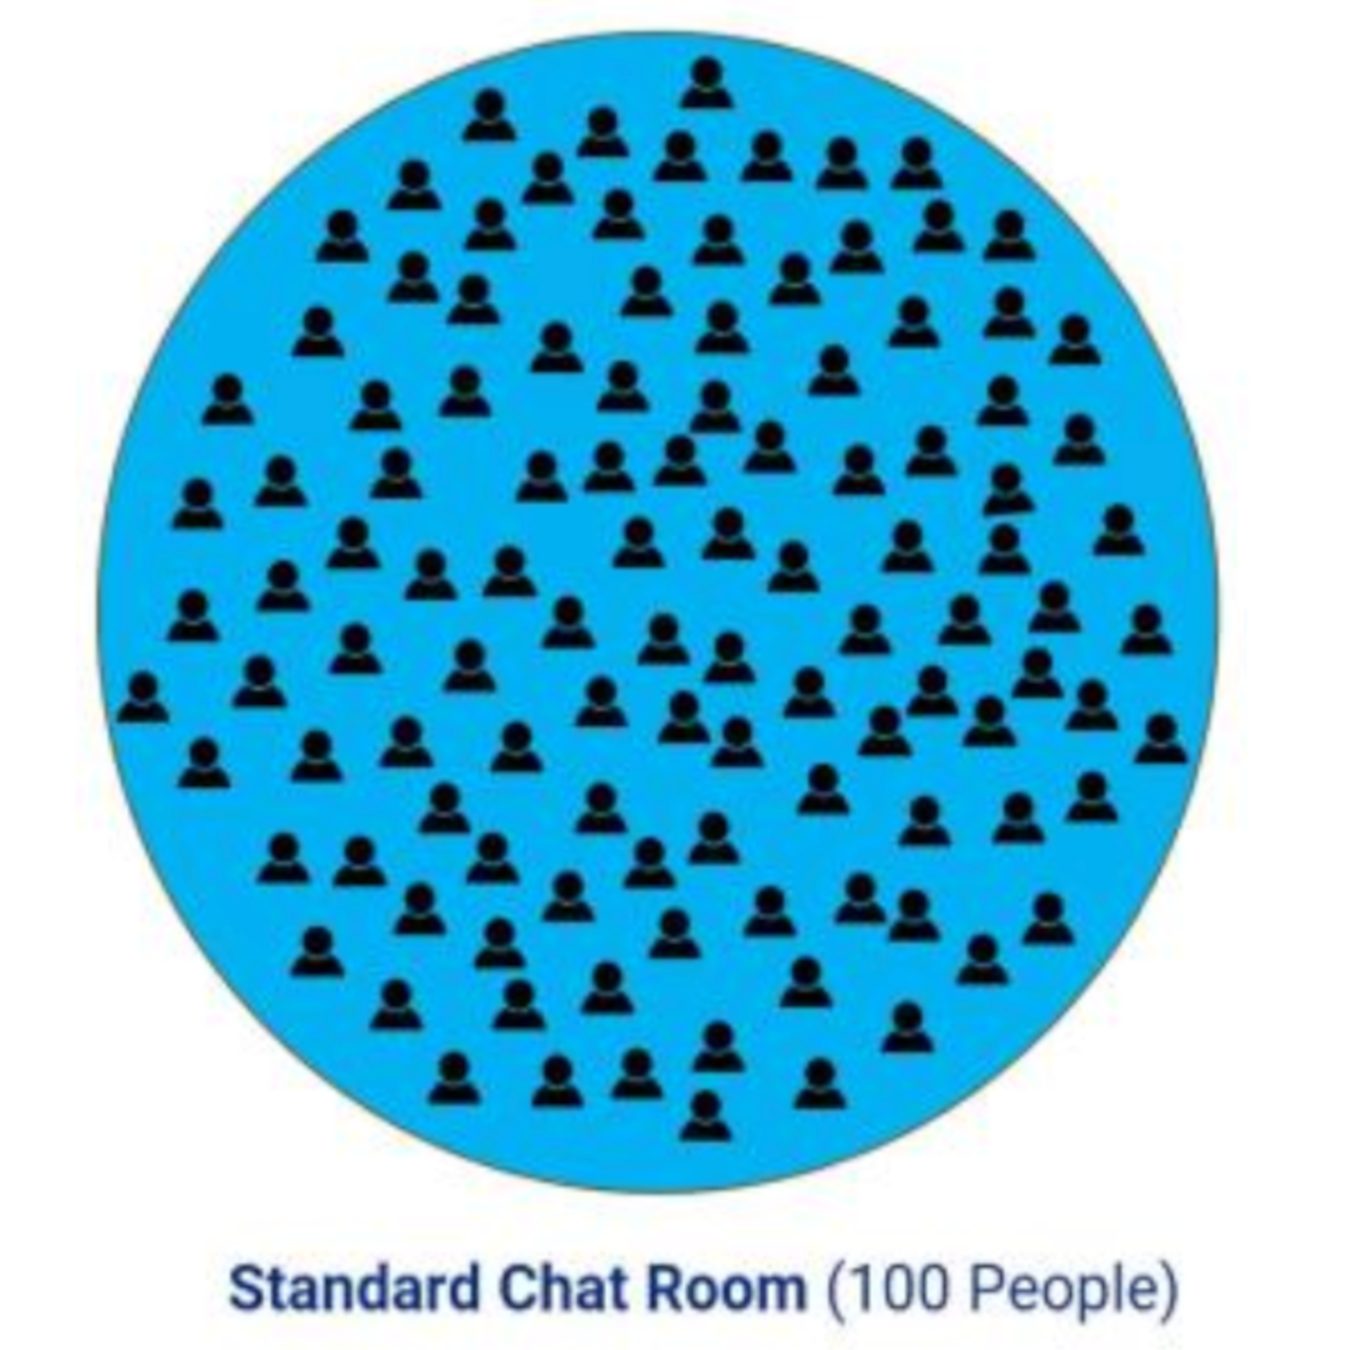
\includegraphics[width=0.8\textwidth]{imgs/CSI_section/standard_chat_room.png}
\end{frame}

\begin{frame}{Conversational Swarm Intelligence}
\vspace{-0.5in}
\begin{enumerate}
    \item Break into 20 groupchats of 5 people
    \item ChatGPT periodically records "insights"
    \item Your insights get sent to other groups
    \item You recieve other groups' insights
    \item Info that sparks discussion will propagate
\end{enumerate}
\centering
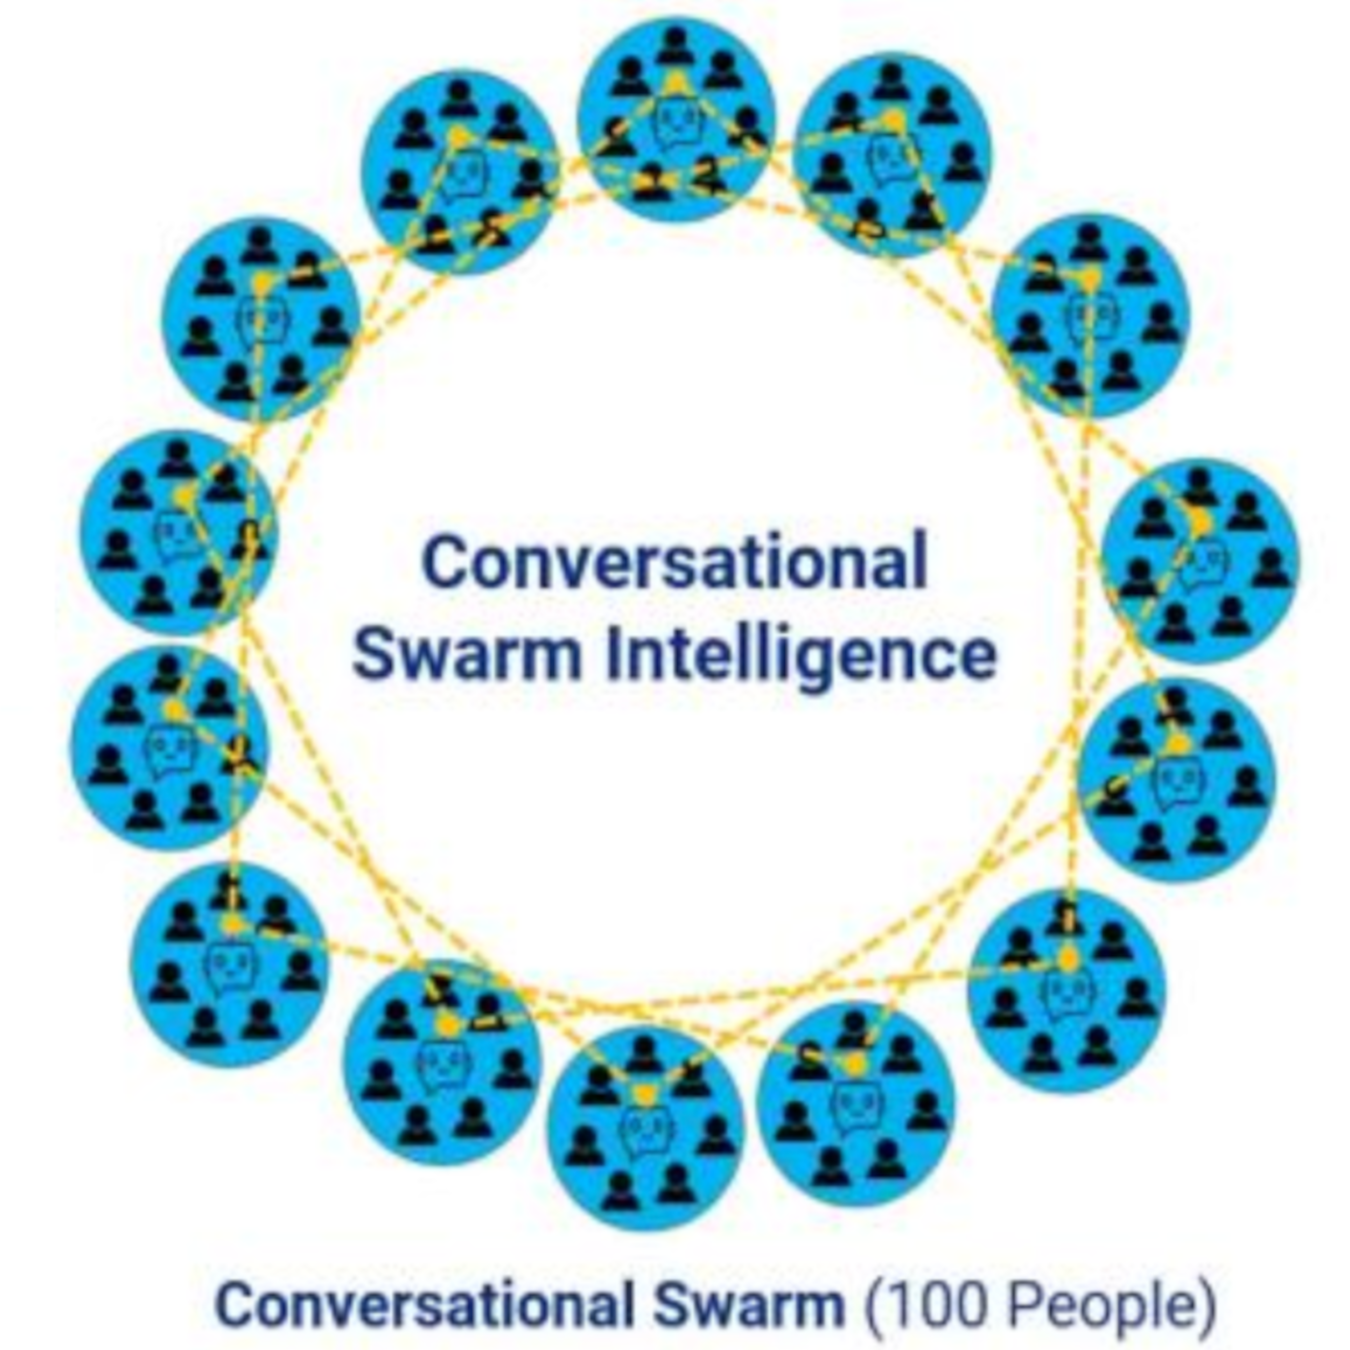
\includegraphics[width=0.8\textwidth]{imgs/CSI_section/conversational_swarm.png}
\end{frame}

\begin{frame}{Credit}
\vspace{-1.5in}
\begin{center}
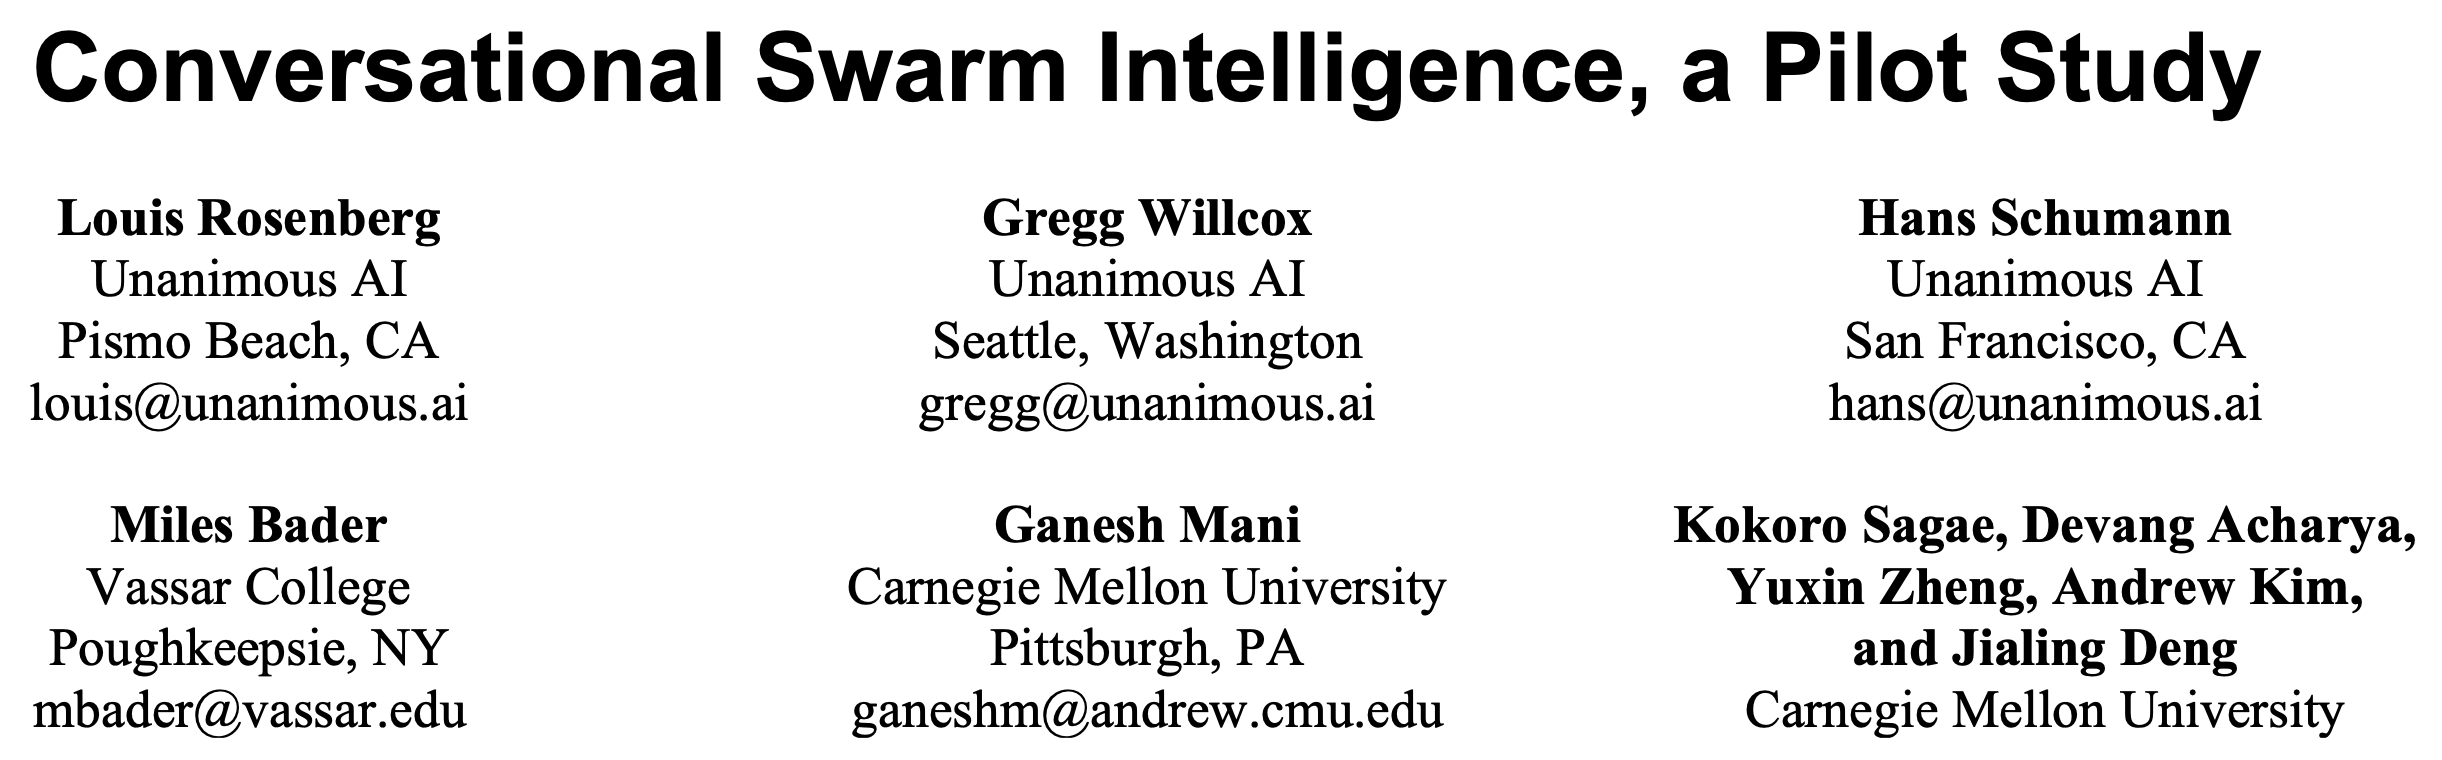
\includegraphics[width=\textwidth]{imgs/CSI_section/authors.png}
\end{center}
\end{frame}

\begin{frame}{Defining "Insights"}
\vspace{-1in}
\begin{itemize}
    \item You can directly edit / take over
    \begin{itemize}
        \item Learns what you prefer over time
    \end{itemize}
    \item Many settings to fiddle with
    \begin{itemize}
        \item frequency
        \item length/detail
        \item group size
        \item what groups will you join?
    \end{itemize}
    \item Customize the insights to your needs
    \begin{itemize}
        \item HistorianGPT: summary
        \item InternGPT: action items
        \item Devil's Advocate: criticisms
        \item personalize to group that's receiving
        \begin{itemize}
            \item architects $\rightarrow$ engineers\\vs\\architects $\rightarrow$ sales team
        \end{itemize}
    \end{itemize}
\end{itemize}
\end{frame}

\begin{frame}{Target Audiences}
\vspace{-0.4in}
\begin{itemize}
    \item Online shared interest communities
    \item Local community organization
    \item Replace middle-management
    \item Grassroots movements won't need leaders or centralized decision making
    \item Literally any large group of people
\end{itemize}
\centering

\includegraphics[width=0.8\textwidth]{imgs/CSI_section/competition.png}
\end{frame}

\begin{frame}{Other Videos}
\centering
\tiny
\vspace{-1.5in}
\begin{itemize}
    \item Part 1: Why replace TikTok?
    \item Part 2: Weird groupchats 
    \item Part 3: Past vertical video
    \item Part 4: Decentralization
    \item Part 5: Redesigned Algorithm
    \item Part 6: Misc / How to help
\end{itemize}
\end{frame}

\begin{frame}
\centering
\vspace{-1in}

\includegraphics[width=0.4\textwidth]{imgs/app_icons/tiktok-icon2.png}\\
TikTok Successor Proposal \\
(Part 3: Beyond Vertical Videos)
\end{frame}

\begin{frame}{What stays the same}
\vspace{-0.7in}
\begin{itemize}
    \item Short-form vertical video still dominant
    \item Algorithm-driven
    \begin{itemize}
        \item More on this in Part 5
    \end{itemize}
\end{itemize}
\centering
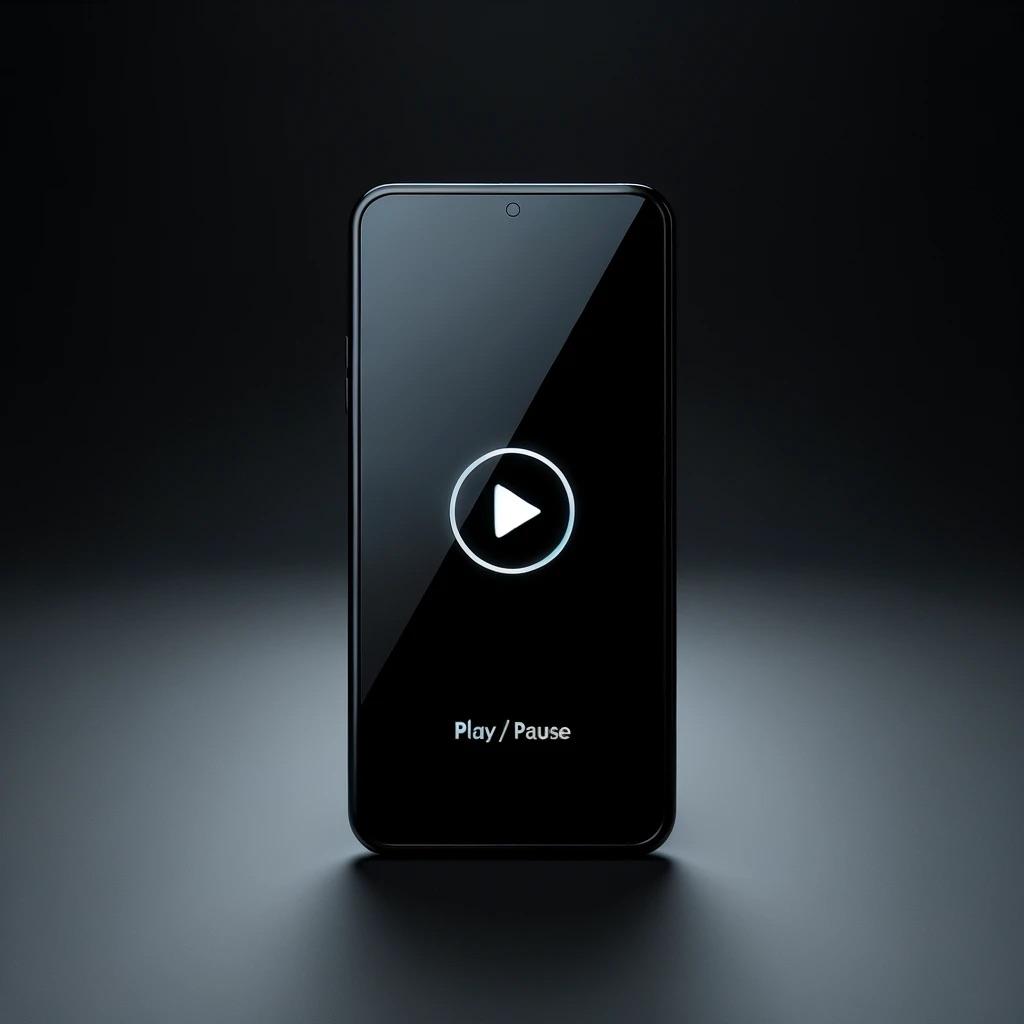
\includegraphics[width=0.8\textwidth]{imgs/media/vertical_vid.jpeg}
\end{frame}

\begin{frame}{Horizontal Video}
\vspace{-0.6in}
\begin{itemize}
    \item Just rotate your phone
        \item Longer-form content
        \item Introduces whole different culture
        \begin{itemize}
            \item higher detail/quality/rigor/length
        \end{itemize}
\end{itemize}
\centering
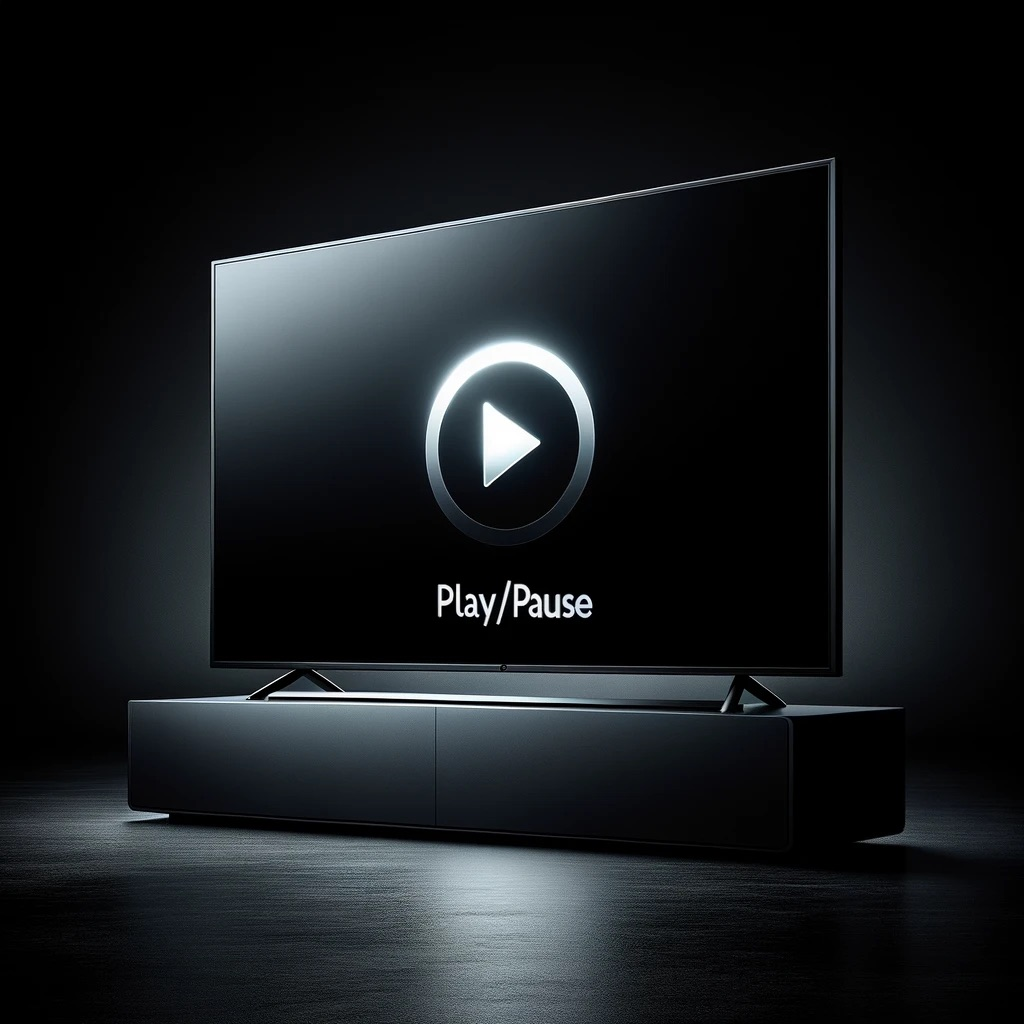
\includegraphics[width=0.8\textwidth]{imgs/media/horizontal_vid.jpeg}
\end{frame}

\begin{frame}{Written Articles}
\vspace{-0.5in}
\begin{itemize}
    \item Include actual links to sources
    \item Invites "legit" (traditional) journalism
    \item Literally just in your FYP feed
    \item Comment/stitch them to videos
    \item TLDR for me, but Nerds will love
    \item Also tweet-length stuff
\end{itemize}
\centering

\includegraphics[width=0.8\textwidth]{imgs/media/quil.png}
\end{frame}

\begin{frame}{Integration w/\\Conversational Swarms}
\vspace{-1.1in}
\begin{itemize}
    \item Watch Part 2 for this to make sense
    \item Alongside your "FYP", each Swarm you're\\in will have its own vertical scroll feed
    \item Livestreamers \textit{(optionally)} talk with a Swarm\\of the viewers instead of chat
    \item In groupchats, a ChatGPT can \textit{(optionally)}\\be on standby to send videos \& articles\\relevant to your conversation
    \begin{itemize}
        \item inspiration
        \item fact-checking
        \item counter-arguments
    \end{itemize}
\end{itemize}
\end{frame}

\begin{frame}{Other Videos}
\centering
\tiny
\vspace{-1.5in}
\begin{itemize}
    \item Part 1: Why replace TikTok?
    \item Part 2: Weird groupchats 
    \item Part 3: Past vertical video
    \item Part 4: Decentralization
    \item Part 5: Redesigned Algorithm
    \item Part 6: Misc / How to help
\end{itemize}
\end{frame}

\begin{frame}
\centering
\vspace{-1in}

\includegraphics[width=0.4\textwidth]{imgs/app_icons/tiktok-icon2.png}\\
TikTok Successor Proposal \\
(Part 4: Power to the Ppl)
\end{frame}

\begin{frame}{Modularity/Choice}
\vspace{-0.3in}
\begin{itemize}
    \item EVERYTHING is optional; \\turn anything off
    \begin{itemize}
        \item Data privacy
        \item May reduce experience
    \end{itemize}
    \item Swap-out features
    \begin{itemize}
        \item Algorithms
        \item GPT in your Swarm
        \begin{itemize}
            \item "Swarm" defined in Part 2
        \end{itemize}
    \end{itemize}
\end{itemize}
\centering

\includegraphics[width=0.8\textwidth]{imgs/power_to_people/legos.png}
\end{frame}

\begin{frame}{Open-Source}
\vspace{-0.7in}
\begin{itemize}
    \item Definition: all code is released to the\\internet, free for anyone to use
    \begin{itemize}
        \item Nerds don't need profit incentive to\\make cool things
    \end{itemize}
    \item Open-source as many parts as possible,\\maybe even whole thing
    \item Companies, organizations, nerds, etc can\\build their own versions
\end{itemize}
\centering

\includegraphics[width=0.8\textwidth]{imgs/power_to_people/open-source.png}
\end{frame}

\begin{frame}{Encryption}
\vspace{-1.4in}
\begin{itemize}
    \item Encryption for privacy wherever possible
    \begin{itemize}
        \item Incompatible with some features;\\some not enabled by default
    \end{itemize}
    \item \emoji{lock} + Swarm $\rightarrow$ competes w/ Telegram
    \begin{itemize}
        \item Run your own local ChatGPT for Conversational Swarm and use it fully encrypted instead of our default model
        \item "Swarm" defined in Part 2
    \end{itemize}
\end{itemize}
\end{frame}

\begin{frame}{Decentralization}
\vspace{-0.4in}
\begin{itemize}
    \item Crypto bros are cringe; that's not this
    \begin{itemize}
        \item No investment currency involved
    \end{itemize}
    \item Underlying technology (blockchain) means\\NO ONE can control your info/activity
    \item The FYP algorithm requires a lot of\\compute to run
    \begin{itemize}
        \item Federated instead of flat
    \end{itemize}
\end{itemize}
\centering
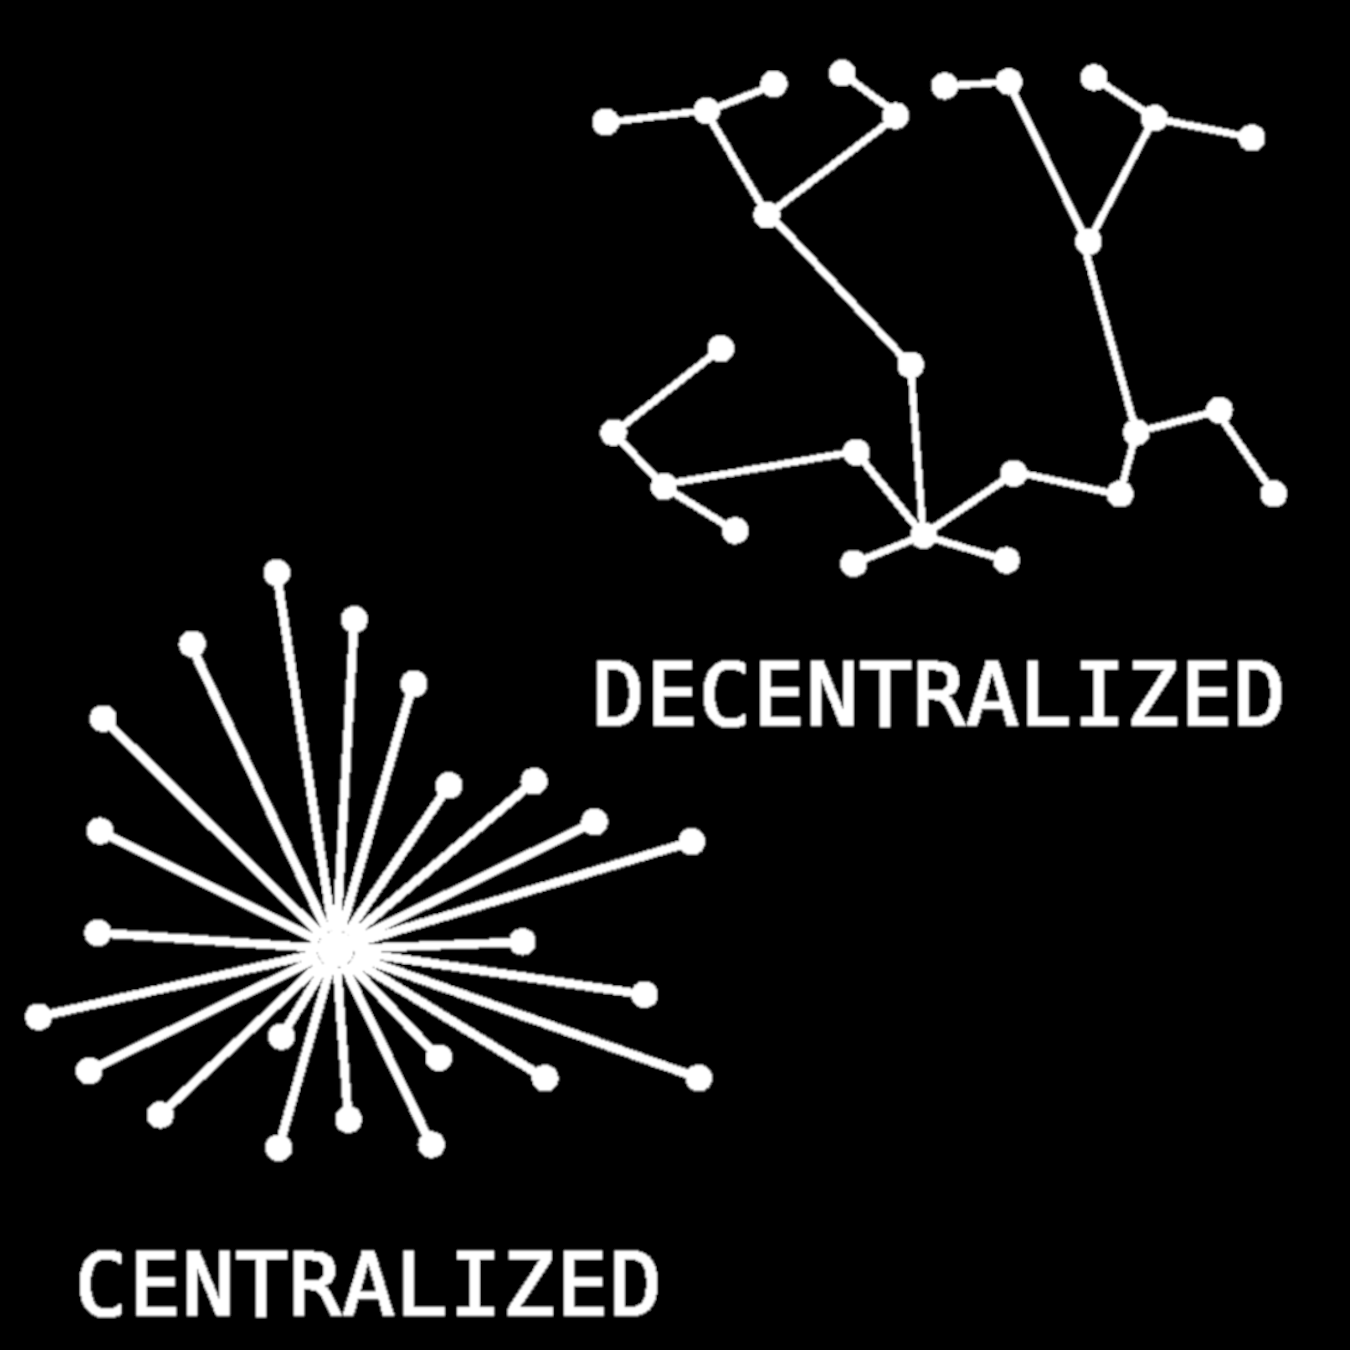
\includegraphics[width=0.8\textwidth]{imgs/power_to_people/decentralized.png}
\end{frame}

\begin{frame}{Other Videos}
\centering
\tiny
\vspace{-1.5in}
\begin{itemize}
    \item Part 1: Why replace TikTok?
    \item Part 2: Weird groupchats 
    \item Part 3: Past vertical video
    \item Part 4: Decentralization
    \item Part 5: Redesigned Algorithm
    \item Part 6: Misc / How to help
\end{itemize}
\end{frame}

\begin{frame}
\centering
\vspace{-1in}

\includegraphics[width=0.4\textwidth]{imgs/app_icons/tiktok-icon2.png}\\
TikTok Successor Proposal \\
(Part 5: Redesigned Algorithm)
\end{frame}

\begin{frame}{Thesis}
\vspace{-1.8in}
\begin{itemize}
    \item Algorithms could be good (less bad)\\if there were no (less) profit incentive
    \item ***My expertise is in AI language models,\\not recommendation algorithms
 \end{itemize}
\end{frame}

\begin{frame}{Current Algorithm Dynamic}
\vspace{-1.4in}
\begin{enumerate}
    \item Companies want \$
    \item Advertising $\rightarrow$ \$
    \item Addicting you $\rightarrow$ more time for ads
    \item Brains respond to sycophantic praise \&\\negative emotions (anger, fear, etc.)
    \item Designed/trained to isolate you into an\\ideological bubble \& make you hate/fear\\people/ideas outside the bubble
\end{enumerate}
\end{frame}

\begin{frame}{TikTok's Algorithm}
\vspace{-1.2in}
\tiny
\hspace{0.2in} Still fundamentally works this way BUT
\begin{enumerate}
    \item Short video $\rightarrow$ more videos seen per hour
    \item More data $\rightarrow$ better algorithm
    \begin{itemize}
        \item Youtube shows what you already like
        \item TikTok introduces you to what you\\didn't know you would like
    \end{itemize}
    \item When a topic reaches critical mass it gets\\shown to people who have not previously\\displayed interest
    \begin{itemize}\item hence awareness of \emoji{watermelon}\end{itemize}
\end{enumerate}
\end{frame}

\begin{frame}{Swap Out Algorithms}
\vspace{-1.6in}
\begin{itemize}
    \item Freedom to choose
    \item Simple ones run on gaming PCs
    \item Big AI algorithms need supercomputers
    \begin{itemize}
        \item Incentivize with the right to serve ads
    \end{itemize}
    \item Also swap ChatGPT models in Swarms
    \begin{itemize}
        \item "Swarm" defined in Part 2
    \end{itemize}
\end{itemize}
\end{frame}

\begin{frame}{Default (My) Algorithm}
\vspace{-1.4in}
\begin{itemize}
    \item Similar to Tiktok's;\\these are \textbf{optional settings:}
    \begin{itemize}
        \item Vids it predicts you will \textit{not} like
        \item Occasionally show random content
        \item Only display local content
        \item Constantly try to change your mind
        \item Optimize for growth of your Swarm
    \end{itemize}
    \item All very TBD, idk exactly what's possible
\end{itemize}
\end{frame}

\begin{frame}{Other Videos}
\centering
\tiny
\vspace{-1.5in}
\begin{itemize}
    \item Part 1: Why replace TikTok?
    \item Part 2: Weird groupchats 
    \item Part 3: Past vertical video
    \item Part 4: Decentralization
    \item Part 5: Redesigned Algorithm
    \item Part 6: Misc / How to help
\end{itemize}
\end{frame}

\begin{frame}
\centering
\vspace{-1in}

\includegraphics[width=0.4\textwidth]{imgs/app_icons/tiktok-icon2.png}\\
TikTok Successor Proposal \\
(Part 6: Misc / How2Help)
\end{frame}

\begin{frame}{Other Videos}
\centering
\tiny
\vspace{-1.5in}
\begin{itemize}
    \item Part 1: Why replace TikTok?
    \item Part 2: Weird groupchats 
    \item Part 3: Past vertical video
    \item Part 4: Decentralization
    \item Part 5: Redesigned Algorithm
    \item Part 6: Misc / How to help
\end{itemize}
\end{frame}

\begin{frame}{Potential Branding}
\vspace{-0.2in}
\hspace{0.2in} {\tiny Inspiration sources for names}
\begin{itemize}
    \item Intelligent swarm behavior in animals
    \item Bee hives
    \item Spider webs
    \item Chorus, harmonics
    \item Communication
    \item Cooperation
\end{itemize}
\hspace{0.2in} {\tiny Example names}
\begin{itemize}
    \item World Web
    \item Tea Hive
    \item Harmonhive
\end{itemize}
\centering
\begin{tabular}{ccc}
    
\includegraphics[width=0.2\textwidth]{imgs/app_icons/7.png} & 
\includegraphics[width=0.2\textwidth]{imgs/app_icons/8.png} & 
\includegraphics[width=0.2\textwidth]{imgs/app_icons/1.png} \\ 
    
\includegraphics[width=0.2\textwidth]{imgs/app_icons/3.png} & 
\includegraphics[width=0.2\textwidth]{imgs/app_icons/4.png} & 
\includegraphics[width=0.2\textwidth]{imgs/app_icons/5.png} \\ 
    
\includegraphics[width=0.2\textwidth]{imgs/app_icons/2.png} & 
\includegraphics[width=0.2\textwidth]{imgs/app_icons/6.png} 
\end{tabular}
\end{frame}

\begin{frame}{Why Did I Post This?}
\vspace{-1.5in}
\begin{itemize}
    \item Please critique, suggest, etc
    \item Ideally community run \& funded
    \begin{itemize}
        \item I don't have access to VC money
    \end{itemize}
    \item I'm holding back on most of the idea
    \begin{itemize}
        \item If you try to beat me to it you're\\only helping me
    \end{itemize}
\end{itemize}
\end{frame}

\begin{frame}{Minimum Viable Products}
\vspace{-1.5in}
\begin{itemize}
    \item Discord bot
    \item Twitch stream
    \item Discord/Telegram/Slack competitor\\(ignore the TikTok/video part)
\end{itemize}
\end{frame}

\begin{frame}{How Can You Help?}
\vspace{-1.5in}
\begin{itemize}
    \item SHARE, stitch your own thoughts/ideas
    \item Link in bio to a google form
    \begin{itemize}
        \item Email list for IF/when app comes out
        \item Contribute labor/code
        \item Contribute funding
        \item Contribute compute
    \end{itemize}
\end{itemize}
\end{frame}

\begin{frame}{Other Videos}
\centering
\tiny
\vspace{-1.5in}
\begin{itemize}
    \item Part 1: Why replace TikTok?
    \item Part 2: Weird groupchats 
    \item Part 3: Past vertical video
    \item Part 4: Decentralization
    \item Part 5: Redesigned Algorithm
    \item Part 6: Misc / How to help
\end{itemize}
\end{frame}

\end{document}
